\scanpage{38}
\margin{37}
commun, i.e. \deleted{tout}\inserted{un} sommet qui est extrémité d'un arc de spéc. exceptionnel, s'appellera arc d'inertie exceptionnel (par abus de langage). Il peut être commode de l'élargir, en modifiant un peu la définition de l'arc de spécialisation exceptionnel, en le faisant s'arrêter un peu avant ses extrémités primitives (disons aux ``milieux des \deleted{l'arc} arêtes \inserted{\deleted{de} constitutives} extrêmes \deleted{(de $\widetilde L$} de l'arc de spécialisation initial) : arc de spécialisation (exceptionnel) ``rétréci''.

\figure{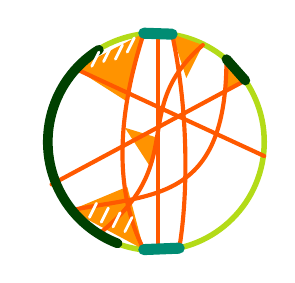
\begin{tikzpicture}[x=.6cm,y=.6cm,line cap=round]
\draw[yellow!70!green,line width=2pt] (0,0) ellipse(2.3 and 2.3);
\fill[orange!85!yellow] (-1.7,1.55)--(-.25,2.3)--(-.6,.85)--cycle;
\fill[orange!85!yellow] (.35,2.28)--(1,2.05)--(.65,1.35)--cycle;
\fill[orange!85!yellow] (1.5,1.75)--(1.9,1.3)--(1.5,1.1)--cycle;
\fill[orange!85!yellow] (-.65,.3)--(0,.1)--(-.1,-.55)--cycle;
\fill[orange!85!yellow] (-1.8,-1.45)--(-.25,-2.28)--(-.6,-.95)--cycle;
\draw[orange!70!red,line width=1.5pt] (-.25,2.3)..controls(-.8,.6)and(-.9,-1)..(-.25,-2.28);
\draw[orange!70!red,line width=1.5pt] (.05,2.3)--(.05,-2.3);
\draw[orange!70!red,line width=1.5pt] (.35,2.28)..controls(.75,.4)and(.65,-1.4)..(.5,-2.25);
\draw[orange!70!red,line width=1.5pt] (-1.7,1.55)--(2.3,-.3);
\draw[orange!70!red,line width=1.5pt] (-2.2,-.9)--(1.9,1.3);
\draw[orange!70!red,line width=1.5pt] (-1.8,-1.45)..controls(-.1,-1.1)and(1.5,-1.3)..(1.5,1.75);
\draw[orange!70!red,line width=1.5pt] (-1.2,-1.95)..controls(.75,-.4)and(-.6,.65)..(1,2.05);
\draw[green!25!black,line width=3.5pt] (-1.2,1.95) arc(122:249:2.3 and 2.3);
\draw[green!25!black,line width=3.5pt] (1.5,1.75)--(1.9,1.3);
\draw[blue!45!green,line width=4pt] (-.25,2.3)--(.35,2.28);
\draw[blue!45!green,line width=4pt] (-.25,-2.28)--(.5,-2.25);
\foreach \x/\y in {-1.35/1.6,-1.1/1.7,-.85/1.75,-.6/1.9,-1.4/-1.6,-1.15/-1.7,-.9/-1.8,-.65/-1.9} {\draw[white,line width=1pt](\x,\y)--+(.15,.3);}
\end{tikzpicture}}
Le bénéfice, c'est que les \unsure{C} les arcs de \deleted{spécialisation}\inserted{transition} sont mutuellement disjoints dans tous les cas, et \inserted{de} deux arcs caractéristiques rétrécis adjacents, \deleted{\unsure{il}} un et un seul est arc de neutralité (au \deleted{sens} ``rétréci''), sans avoir à faire d'exception.

Comme le nom l'indique, les arcs de générisation servent à \deleted{\unsure{définir}} \inserted{réaliser} une opération de générisation, qui consiste à ``croiser les brins'' au dessus dudit arc, de façon que lui et son antipodique cessent d'être arcs de générisation.

\figure{\begin{tikzpicture}[x=.52cm,y=.52cm,line cap=round]
\draw[yellow!70!green,line width=2pt] (0,0) ellipse(1.65 and 1.65);
\fill[orange!85!yellow] (-1.4,1)--(-.85,.25)--(-1.65,.3)--cycle;
\fill[orange!85!yellow] (-.45,.1)--(-.15,-.4)--(.35,-.2)--cycle;
\draw[orange!70!red,line width=1.5pt] (-.1,1.65)..controls(-.8,.2)and(-.8,-.4)..(-.2,-1.65);
\draw[orange!70!red,line width=1.5pt] (.3,1.63)..controls(.8,.3)and(.5,-.9)..(.15,-1.65);
\draw[orange!70!red,line width=1.5pt] (-1.65,.3)..controls(-.3,.7)and(.9,.3)..(1.65,-.1);
\draw[orange!70!red,line width=1.5pt] (-1.4,1)--(-.8,.2)--(1.55,-.65);
\draw[orange!70!red,line width=1.5pt] (-1.55,-.85)..controls(-.1,-.5)and(.9,.65)..(1.4,1);
\draw[green!30!black,line width=3pt](-.1,1.65)--(.3,1.63);\draw[green!30!black,line width=3pt](-.2,-1.65)--(.15,-1.65);
\node[above]at(-.2,1.7){$D$};\node[above]at(.35,1.7){$D'$};\node[below]at(-.3,-1.7){$D$};\node[below]at(.3,-1.7){$D'$};
\draw[|->] (2,.1)--(2.65,.1);\draw[|->](2.65,-.55)--(2,-.55);
\node[inner sep=0pt] at (4.5,0) {\deleted{\begin{tikzpicture}[x=.52cm,y=.52cm,line cap=round]
\draw[yellow!70!green,line width=2pt](0,0)ellipse(1.5 and 1.7);
\draw[orange!70!red,line width=1.5pt](-.3,1.7)..controls(-.2,.2)and(.3,-.8)..(.55,-1.6);
\draw[orange!70!red,line width=1.5pt](.4,1.65)..controls(.4,.3)and(.5,-.7)..(-.15,-1.7);
\draw[orange!70!red,line width=1.5pt](-1.45,.3)--(1.45,-.3);
\draw[orange!70!red,line width=1.5pt](-1.4,-.55)--(1.2,1.1);
\draw[orange!70!red,line width=1.5pt](-1.4,.3)--(-.45,1.9)--(-1.1,-.85)--(.2,1.7)--(-.6,-.9)--(1.1,.4)--(.2,-1.15)--(1,-.9)--(.6,-1.5);
\draw[black,line width=.8pt](-1.35,.35)--(-.25,1.9)--(-1.3,-.55)--(.3,1.9)--(-.6,-1)--(.7,1.6)--(-.1,-1.1)--(1.2,.8)--(.5,-1.3)--(1.05,-.7)--(.7,-1.5);
\end{tikzpicture}}};
\begin{scope}[shift={(7.7,.3)}]
\draw[yellow!70!green,line width=2pt](0,0)ellipse(1.75 and 1.7);
\fill[orange!85!yellow](-1.5,1)--(-.9,.4)--(-1.7,.05)--cycle;
\draw[orange!70!red,line width=1.5pt](-.1,1.7)..controls(-.2,.5)and(-.6,-1.4)..(.1,-1.7);
\draw[orange!70!red,line width=1.5pt](.35,1.65)..controls(.5,.1)and(.4,-1)..(-.35,-1.65);
\draw[orange!70!red,line width=1.5pt](.65,1.6)..controls(1,.5)and(1,-.7)..(-.35,-1.65);
\draw[orange!70!red,line width=1.5pt](-1.75,.05)..controls(-.5,.7)and(.6,.25)..(1.75,-.2);
\draw[orange!70!red,line width=1.5pt](-1.5,1)--(-.9,.4)--(1.7,-.55);
\draw[orange!70!red,line width=1.5pt](-1.4,-1.1)..controls(0,-1)and(.8,.7)..(1.45,.95);
\draw[green!30!black,line width=3pt](-.35,-1.65)--(.1,-1.7);
\node[above]at(-.2,1.7){$D$};\node[above]at(.45,1.7){$D'$};\node[below]at(-.45,-1.75){$D'$};\node[below]at(.2,-1.75){$D$};
\end{scope}
\end{tikzpicture}}

(\uline{NB} Le polygone structural $\widetilde L$, à isom comb. canonique près, n'aura pas changé) par contre l'arc en question est devenu arc de spécialisation. Dans $X$, l'opération se visualise comme un antibalayage, en \uline{décollant} le sommet $s$ de $\overline\Sigma$ dans la direction opposée : celle où se trouve \unsure{l'arc} de générisation, qui ``pousse'' sur $L$, et en joignant $L$, donne l'arc de spécialisation correspondant.

\figure{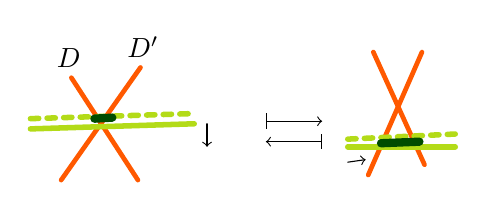
\begin{tikzpicture}[x=.65cm,y=.65cm,line cap=round]
\draw[orange!70!red,line width=1.7pt](-.8,1)--(.5,-1);\draw[orange!70!red,line width=1.7pt](.55,1.2)--(-1,-1);
\draw[yellow!70!green,line width=2pt](-1.6,0)--(1.6,.1);\draw[yellow!70!green,dashed,line width=2pt](-1.6,.2)--(1.6,.3);
\draw[green!30!black,line width=3pt](-.35,.2)--(0,.22);
\node[above]at(-.85,1){$D$};\node[above]at(.6,1.2){$D'$};\draw[->](1.85,.1)--(1.85,-.35);
\draw[|->](3,.15)--(4.1,.15);\draw[|->](4.1,-.25)--(3,-.25);
\begin{scope}[shift={(5.7,0)}]
\draw[orange!70!red,line width=1.7pt](-.6,1.5)--(.4,-.7);\draw[orange!70!red,line width=1.7pt](.35,1.5)--(-.7,-.9);
\draw[yellow!70!green,line width=2pt](-1.1,-.35)--(1,-.35);\draw[yellow!70!green,dashed,line width=2pt](-1.1,-.2)--(1,-.1);
\draw[green!30!black,line width=3pt](-.45,-.28)--(.3,-.25);\draw[->](-1.1,-.65)--(-.75,-.6);
\end{scope}
\end{tikzpicture}}
Ceci dit, si $(L,a)$ et $(L',a')$ ($a$ arc de gén. de $L$, $a'$ arc de spécialisation de $L'$) se correspondent, il est utile d'\uline{attacher} $\Delta_L$ \uline{à} $\Delta_{L'}$, par identification de $a$ avec $a'$, par un isom lin. affine

\figure{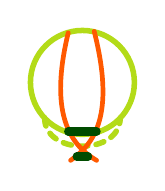
\begin{tikzpicture}[x=.6cm,y=.6cm,line cap=round]
\draw[yellow!70!green,line width=2pt](0,0)ellipse(1.1 and 1.1);
\draw[yellow!70!green,dashed,line width=2pt](-.8,-.75)..controls(-.8,-1.55)and(.8,-1.55)..(.8,-.75);
\draw[orange!70!red,line width=1.7pt](-.3,1.05)..controls(-.7,-.6)and(-.3,-1.3)..(.3,-1.65);
\draw[orange!70!red,line width=1.7pt](.25,1.08)..controls(.7,-.7)and(.25,-1.3)..(-.25,-1.65);
\draw[green!30!black,line width=3pt](-.3,-1.04)--(.3,-1.04);\draw[green!30!black,line width=3pt](-.12,-1.57)--(.12,-1.57);
\end{tikzpicture}}
